%% For double-blind review submission, w/o CCS and ACM Reference (max submission space)
\documentclass[sigplan,review,anonymous]{acmart}\settopmatter{printfolios=true,printccs=false,printacmref=false}
%% For double-blind review submission, w/ CCS and ACM Reference
%\documentclass[sigplan,review,anonymous]{acmart}\settopmatter{printfolios=true}
%% For single-blind review submission, w/o CCS and ACM Reference (max submission space)
%\documentclass[sigplan,review]{acmart}\settopmatter{printfolios=true,printccs=false,printacmref=false}
%% For single-blind review submission, w/ CCS and ACM Reference
%\documentclass[sigplan,review]{acmart}\settopmatter{printfolios=true}
%% For final camera-ready submission, w/ required CCS and ACM Reference
%\documentclass[sigplan]{acmart}\settopmatter{}

\usepackage{kantlipsum}
\usepackage{enumitem}
\usepackage{multirow}
\usepackage{hhline}
\usepackage{caption}
\usepackage{makecell}
\usepackage{ragged2e}
\usepackage{parskip}
\usepackage{wrapfig}
\usepackage{array}
\usepackage{float}
\usepackage[english]{babel}
\usepackage{lipsum}
\usepackage{caption}
\usepackage{subcaption}
\usepackage{graphicx}
\graphicspath{{images/}} 
\usepackage[linesnumbered,ruled]{algorithm2e}
\usepackage{courier}
\usepackage{hyperref}
\hypersetup{colorlinks=true,allcolors=blue}
\usepackage{listings}
\lstset{
    basicstyle=\ttfamily,
    frame=none, 
    breaklines=true,
    numbers=left,
    xleftmargin=2.5em,
    framexleftmargin=0em,
    emphstyle=\textbf,
    float=t
}
\lstdefinestyle{ocl}{
    emph={
        context, inv
    }
}
\lstdefinestyle{cbp}{
    basicstyle=\ttfamily\scriptsize,
    emph={
        session, create, of, type,
        set, to, add, hire
    }
}
\lstdefinestyle{xmi}{
    basicstyle=\ttfamily\scriptsize,
    emph={
        Node, children
    }
}
\lstdefinestyle{xml}{
    basicstyle=\ttfamily\scriptsize,
    emph={
        register, create, add, to, resource,
        from, eattribute, remove, ereference,
        set, unset, session, Roy, Jen,
        Moss, Richmond
    }
}
\lstdefinestyle{java}{
    basicstyle=\ttfamily\scriptsize,
    emph={
        case, $unset$,
        instanceof, else, if, void,
        new, UnsetEAttributeEvent,
        UnsetEReferenceEvent,
        @override, public, class, extends
    }
}
\lstdefinestyle{eol}{
    basicstyle=\ttfamily\scriptsize,
    emph={
        var, new, for, in, create, set, of, with, type,
        unset, to, add, remove, delete, register, move,
        from, position, from, move-within, session, \.
    }
}


\hyphenation{op-tical net-works semi-conduc-tor Change-Hybrid-Event-Adapter Change-Hybrid-XMI-Event-Adapater
    Change-Hybrid-Neo-EMF-Event-Adapater change-Events Change-Event-Adapter EContent-Adapter notify-Changed Hybrid-Resource Resource-Impl state-Based-Resource cbp-Output-Stream Output-Stream Hybrid-Change-Event-Adapater Output-Stream Hybrid-XMI-Resource-Impl Hybrid-Neo-EMF-Resource-Impl Persistence-Resource pack-a-ged-E-le-ment
}

%% Conference information
%% Supplied to authors by publisher for camera-ready submission;
%% use defaults for review submission.
\acmConference[ACM SRC@MODELS'18]{ACM Student Research Competition @ MODELS 2018}{October 14-19, 2018}{Copenhagen, Denmark}
\acmYear{2018}
\acmISBN{} % \acmISBN{978-x-xxxx-xxxx-x/YY/MM}
\acmDOI{} % \acmDOI{10.1145/nnnnnnn.nnnnnnn}
\startPage{1}

%% Copyright information
%% Supplied to authors (based on authors' rights management selection;
%% see authors.acm.org) by publisher for camera-ready submission;
%% use 'none' for review submission.
\setcopyright{none}
%\setcopyright{acmcopyright}
%\setcopyright{acmlicensed}
%\setcopyright{rightsretained}
%\copyrightyear{2018}           %% If different from \acmYear

%% Bibliography style
\bibliographystyle{ACM-Reference-Format}
%% Citation style
%\citestyle{acmauthoryear}  %% For author/year citations
%\citestyle{acmnumeric}     %% For numeric citations
%\setcitestyle{nosort}      %% With 'acmnumeric', to disable automatic
                            %% sorting of references within a single citation;
                            %% e.g., \cite{Smith99,Carpenter05,Baker12}
                            %% rendered as [14,5,2] rather than [2,5,14].
%\setcitesyle{nocompress}   %% With 'acmnumeric', to disable automatic
                            %% compression of sequential references within a
                            %% single citation;
                            %% e.g., \cite{Baker12,Baker14,Baker16}
                            %% rendered as [2,3,4] rather than [2-4].


%%%%%%%%%%%%%%%%%%%%%%%%%%%%%%%%%%%%%%%%%%%%%%%%%%%%%%%%%%%%%%%%%%%%%%
%% Note: Authors migrating a paper from traditional SIGPLAN
%% proceedings format to PACMPL format must update the
%% '\documentclass' and topmatter commands above; see
%% 'acmart-pacmpl-template.tex'.
%%%%%%%%%%%%%%%%%%%%%%%%%%%%%%%%%%%%%%%%%%%%%%%%%%%%%%%%%%%%%%%%%%%%%%


%% Some recommended packages.
\usepackage{booktabs}   %% For formal tables:
                        %% http://ctan.org/pkg/booktabs
\usepackage{subcaption} %% For complex figures with subfigures/subcaptions
                        %% http://ctan.org/pkg/subcaption


\begin{document}

%% Title information
\title[Short Title]{Change-based Persistence}         %% [Short Title] is optional;
                                        %% when present, will be used in
                                        %% header instead of Full Title.
%\titlenote{with title note}             %% \titlenote is optional;
                                        %% can be repeated if necessary;
                                        %% contents suppressed with 'anonymous'
%\subtitle{Subtitle}                     %% \subtitle is optional
%\subtitlenote{with subtitle note}       %% \subtitlenote is optional;
                                        %% can be repeated if necessary;
                                        %% contents suppressed with 'anonymous'


%% Author information
%% Contents and number of authors suppressed with 'anonymous'.
%% Each author should be introduced by \author, followed by
%% \authornote (optional), \orcid (optional), \affiliation, and
%% \email.
%% An author may have multiple affiliations and/or emails; repeat the
%% appropriate command.
%% Many elements are not rendered, but should be provided for metadata
%% extraction tools.

%% Author with single affiliation.
\author{Alfa Yohannis}
\authornote{with author1 note}          %% \authornote is optional;
                                        %% can be repeated if necessary
\orcid{0000-0003-4425-3731}             %% \orcid is optional
\affiliation{
  \position{Research Student}
  \department{Computer Science Department}              %% \department is recommended
  \institution{University of York}            %% \institution is required
  \streetaddress{Heslington East}
  \city{York}
  \state{North Yorkshire}
  \postcode{YO10 5GE}
  \country{United Kingdom}                    %% \country is recommended
}
\email{first1.last1@inst1.edu}          %% \email is recommended

\affiliation{
    \position{Research Student}
    \department{Computer Science Department}              %% \department is recommended
    \institution{Institut Teknologi dan Bisnis Kalbis}            %% \institution is required
    \streetaddress{Jl. Pulomas Selatan kav.22}
    \city{Jakarta Timur}
    \state{DKI Jakarta}
    \postcode{13210}
    \country{Indonesia}                    %% \country is recommended
}
\email{alfa.yohannis@kalbis.ac.id}          %% \email is recommended

%%% Author with two affiliations and emails.
%\author{First2 Last2}
%\authornote{with author2 note}          %% \authornote is optional;
%                                        %% can be repeated if necessary
%\orcid{nnnn-nnnn-nnnn-nnnn}             %% \orcid is optional
%\affiliation{
%  \position{Position2a}
%  \department{Department2a}             %% \department is recommended
%  \institution{Institution2a}           %% \institution is required
%  \streetaddress{Street2a Address2a}
%  \city{City2a}
%  \state{State2a}
%  \postcode{Post-Code2a}
%  \country{Country2a}                   %% \country is recommended
%}
%\email{first2.last2@inst2a.com}         %% \email is recommended
%\affiliation{
%  \position{Position2b}
%  \department{Department2b}             %% \department is recommended
%  \institution{Institution2b}           %% \institution is required
%  \streetaddress{Street3b Address2b}
%  \city{City2b}
%  \state{State2b}
%  \postcode{Post-Code2b}
%  \country{Country2b}                   %% \country is recommended
%}
%\email{first2.last2@inst2b.org}         %% \email is recommended


%% Abstract
%% Note: \begin{abstract}...\end{abstract} environment must come
%% before \maketitle command
\begin{abstract}
Change-based persistence has the potential to support faster and more accurate model comparison, merging, as well as a range of analytics activities compared to state-based persistence. However, it also comes with side-effects, such as the increased loading time and ever-growing file size. This paper presents our change-based persistence implementation as well as our solutions to reduce the side-effects. The evaluation results are also presented in this paper. 
\end{abstract}


%% 2012 ACM Computing Classification System (CSS) concepts
%% Generate at 'http://dl.acm.org/ccs/ccs.cfm'.
\begin{CCSXML}
    <ccs2012>
    <concept>
    <concept_id>10011007.10010940.10010971.10010980.10010984</concept_id>
    <concept_desc>Software and its engineering~Model-driven software engineering</concept_desc>
    <concept_significance>500</concept_significance>
    </concept>
    <concept>
    <concept_id>10011007.10010940.10011003.10011002</concept_id>
    <concept_desc>Software and its engineering~Software performance</concept_desc>
    <concept_significance>300</concept_significance>
    </concept>
    <concept>
    <concept_id>10011007.10010940.10010971.10010972</concept_id>
    <concept_desc>Software and its engineering~Software architectures</concept_desc>
    <concept_significance>100</concept_significance>
    </concept>
    </ccs2012>
\end{CCSXML}

\ccsdesc[500]{Software and its engineering~Model-driven software engineering}
\ccsdesc[300]{Software and its engineering~Software performance}
\ccsdesc[100]{Software and its engineering~Software architectures}
%% End of generated code


%% Keywords
%% comma separated list
\keywords{change-based persistence, state-based persistence, model persistence, model comparison and merging}  %% \keywords are mandatory in final camera-ready submission


%% \maketitle
%% Note: \maketitle command must come after title commands, author
%% commands, abstract environment, Computing Classification System
%% environment and commands, and keywords command.
\maketitle


\section{Introduction: Background, motivation, research problem}
\label{ch:introduction}

Most of the models in the context of Model-Driven Engineering are persisted in state-based formats. In such approach, model files contain snapshots of the models' contents, and activities like version control and model comparison to support collaborative modelling are left to external systems such as file-based version-control systems and model differencing facilities. Activities such as change-detection (identifying parts that have changed in a model compared to a previous version) and model comparison (finding differences between models) are computationally consuming for state-based models \cite{Kolovos:2009:DMM:1564596.1564641}. Thus, a new approach is needed to make the computation more efficient.

As an alternative to state-based persistence (SBP), this work proposes that a model can also be persisted in a change-based format, which persists the full sequence of \emph{changes} made to the model instead. The concept of change-based persistence (CBP) is not new and has been used in persisting changes to software, object-oriented databases, and hierarchical documents \cite{DBLP:journals/entcs/RobbesL07,DBLP:conf/sde/LippeO92,DBLP:conf/caise/IgnatN05}. The change-based approach can improve detecting differences more precisely at the semantic level -- that is by providing finer-granularity information (e.g. types of changes, the order of the changes, elements that were changed, previous values, etc.) -- and therefore provide support to resolve them \cite{mens2002state}. The ordered nature of CBP means that changes made to a model can be identified sequentially without having to explore and compare all elements between compared models. Based on these arguments, this work aims to answer this hypothesis, \textit{Change-based persistence reduces the execution time of model change-detection, model comparison, and model merging for large models compared to their execution time in CBP, with acceptable trade-offs on loading and persisting time, memory footprint, and storage space consumption}. This work also explores the advantages and shortcomings of CBP as an alternative approach to CBP for models conforming to 3-layer metamodelling architectures such as EMF and MOF. Persisting models in a change-based format can bring a number of envisioned benefits over CBP, such as the ability to detect changes much faster and more precisely, which can then have positive knock-on effects on supporting (1) developers compare and merge models in collaborative modelling environments, and (2) incremental model management (e.g. incremental query \cite{DBLP:conf/ecmdafa/RathHV12} and model-to-text transformation \cite{DBLP:conf/ecmdafa/OgunyomiRK15}). 

Nevertheless, CBP also comes with downsides, such as ever-growing model files \cite{DBLP:journals/entcs/RobbesL07,DBLP:conf/edoc/KoegelHLHD10} and increased model loading time \cite{mens2002state} which increase storage and computation costs. A model that is frequently modified will increase considerably in file size since every change is added to the file. The increased file size (proportional to the number of persisted changes) will, in turn, increase the loading time of the model since all changes have to be replayed to reconstruct the model's eventual state. These downsides have to be mitigated to enable the practical adoption of CBP. One approach to reducing the file size of change-based models is by removing changes that do not affect the eventual state of the model. For the increased loading time, it can be mitigated by ignoring -- i.e. not replaying -- changes that are cancelled out by later changes or employing change-based and CBP side-by-side so that the benefits of CBP on loading time can be obtained. Other downsides are CBP requires integration with existing tools -- since it is still a non-standard approach -- for its adoption \cite{koegel2010emfstore}, and still has limited support for standard, text-based version controls for collaborative development \cite{koegel2010emfstore}. These downsides can be addressed by developing a CBP plugin for a specific development environment (e.g. Eclipse) and persisting changes in text-based format to support text-based version controls (e.g. Git, SVN).


\section{Related Work}
\label{sec:related_work}
Compared to CBP, instead of persisting states of models, CBP persist the changes of models. This is feasible since modelling platforms (e.g. EMF) already provided notification facilities that inform changes of a model, instead of having to compare the model to its previous version to identify the differences. Th notification approach has been used in several incremental projects, such as IncQuery \cite{DBLP:conf/ecmdafa/RathHV12} and ReactiveATL \cite{DBLP:conf/ecmdafa/OgunyomiRK15}, while the model differencing approach has been provided by model differencing tools, such as SiDiff \cite{kelter2005generic} and EMF Compare \cite{eclipse2017compare}.

Most of the available model persistence products persist models in state-based. For example, EMF persists models in a common standard XMI-formatted text file. EMF Teneo \cite{eclipse2017teneo} persists EMF models in relational databases, while Morsa \cite{DBLP:conf/models/Espinazo-PaganCM11} and NeoEMF \cite{daniel2016neoemf} persist models in document and graph databases, respectively. Regarding collaborative modelling, none of these state-based approaches provides built-in support for versioning and models are eventually stored in binary files/folders which are known to be a poor fit for text-oriented version control systems like Git and SVN. Connected Data Objects (CDO) \cite{eclipse2017cdo}, which provides support for database-backed model persistence, also provides collaboration facilities, but CDO adoption necessitates the use of a separate version control system (e.g. a Git repository for code and a CDO repository for models), which introduces fragmentation and administration challenges \cite{barmpis2014evaluation}. So far, this work only identified EMFStore \cite{koegel2010emfstore} as a product that persists models using change-based approach and uses its own model-specific version control system for collaborative modelling.

While state-based approach offers some advantages compared to change-based approach, such as faster for loading large models \cite{DBLP:conf/models/Espinazo-PaganCM11,daniel2016neoemf}, supported by standard version controls (e.g. GitHub) \cite{koegel2010emfstore}, and a default standard (no need integration with existing tools) \cite{koegel2010emfstore}, it also has a drawback when it comes to model comparison: slower model comparison \cite{DBLP:conf/edoc/KoegelHLHD10} and less accurate since it does not carry more information \cite{mens2002state,DBLP:conf/edoc/KoegelHLHD10} compared to change-based approach. Change-based approach comes with some notable advantages over state-based approach, such as faster \cite{DBLP:conf/sde/LippeO92,DBLP:conf/caise/IgnatN05,DBLP:conf/edoc/KoegelHLHD10} and more accurate \cite{DBLP:journals/entcs/RobbesL07,DBLP:conf/sde/LippeO92,DBLP:conf/caise/IgnatN05,mens2002state} model comparison and merging, and information carried is useful for analytics \cite{DBLP:journals/entcs/RobbesL07}. However, it also comes with side effects, such as increased record size \cite{DBLP:journals/entcs/RobbesL07,DBLP:conf/edoc/KoegelHLHD10}, inefficient for replaying (loading) for long records \cite{mens2002state}, limited supports for standard, text-based version controls (e.g. GitHub) \cite{koegel2010emfstore}, and a non-standard approach (need integration with existing tools) \cite{koegel2010emfstore}.

\section{Approach}

\subsection{Change-based Persistence}
To explain the differences between CBP and CBP, consider a modelling activity on a UML model as presented Fig. \ref{fig:illustration_cbp}. The sub-figures \ref{fig:illustration_3} to \ref{fig:illustration_8} depict the evolution of a UML model at different time stamps. Classes are created and added/removed from \texttt{Package X}. In CBP, only the final state of the model is persisted. Thus, to represent the final state of the UML model, only the information about \texttt{Package X} and \texttt{Class C} needs to be persisted, as presented in Listing \ref{lst:xmimodel2} (XMI format). In CBP all the changes in the model are persisted. Thus, a list of all the events generated along the modification of the model is needed to represent the final state of the model.

\begin{figure}[t]
    \begin{subfigure}[t]{0.49\linewidth}
        \centering
        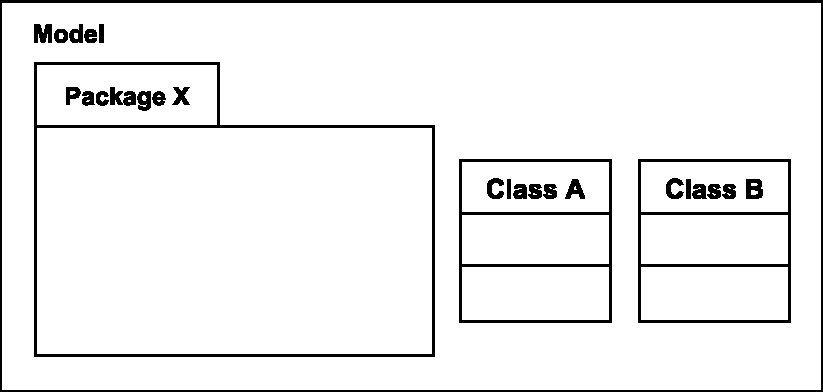
\includegraphics[width=\linewidth]{images/illustration_3}
        \caption{Time stamp 1}
        \label{fig:illustration_3}
    \end{subfigure}
    \begin{subfigure}[t]{0.49\linewidth}
        \centering
        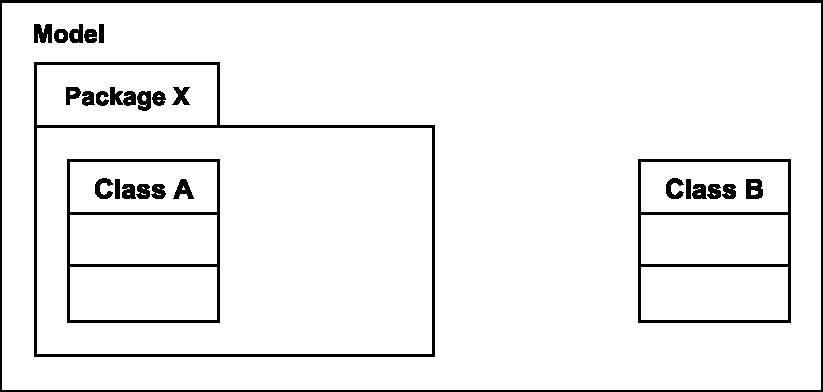
\includegraphics[width=\linewidth]{images/illustration_4}
        \caption{Time stamp 2}
        \label{fig:illustration_4}
    \end{subfigure}
    \hfill
    \begin{subfigure}[t]{0.49\linewidth}
        \centering
        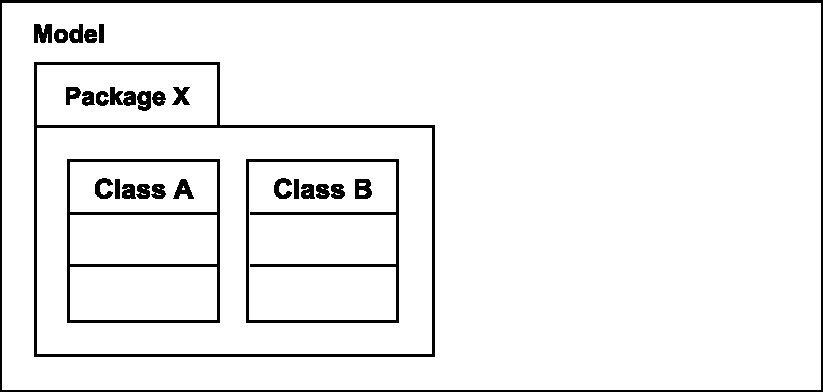
\includegraphics[width=\linewidth]{images/illustration_5}
        \caption{Time stamp 3}
        \label{fig:illustration_5}
    \end{subfigure}
    \begin{subfigure}[t]{0.49\linewidth}
        \centering
        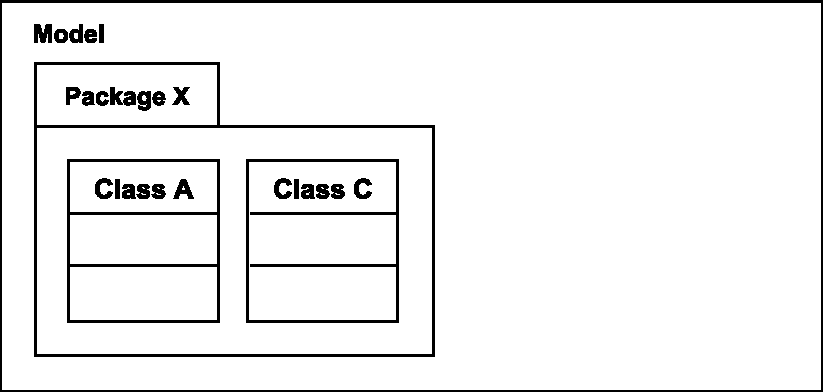
\includegraphics[width=\linewidth]{images/illustration_6}
        \caption{Time stamp 4}
        \label{fig:illustration_6}
    \end{subfigure}
    \hfill
    \begin{subfigure}[t]{0.49\linewidth}
        \centering
        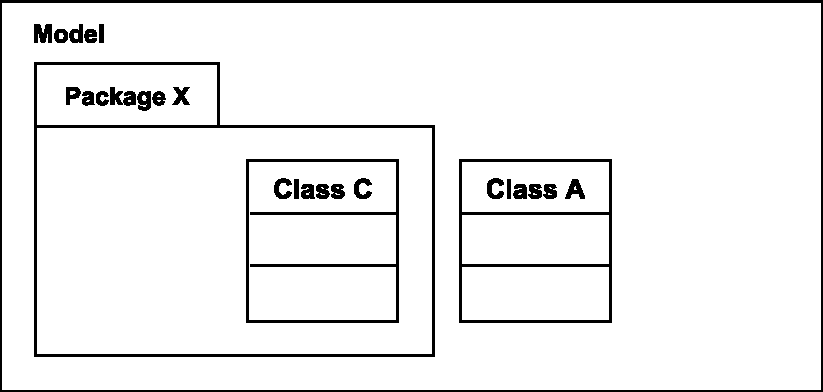
\includegraphics[width=\linewidth]{images/illustration_7}
        \caption{Time stamp 5}
        \label{fig:illustration_7}
    \end{subfigure}
    \begin{subfigure}[t]{0.49\linewidth}
        \centering
        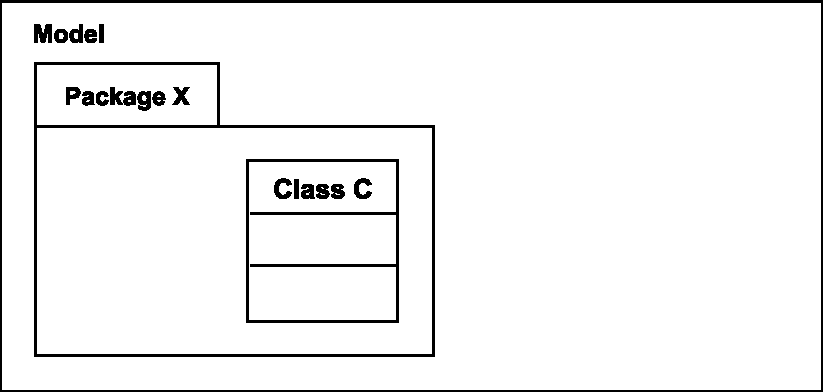
\includegraphics[width=\linewidth]{images/illustration_8}
        \caption{Time stamp 6}
        \label{fig:illustration_8}
    \end{subfigure}
    
    \caption{The states of the example model after certain changes and their corresponding lines in Listing \ref{lst:cbpmodel}.}
    \label{fig:illustration_cbp}
\end{figure}

A session depicts a set of changes made between $save$ events, i.e. a session comprises all the changes that happened since the last time that the model was persisted. The CBP representation is shown in Listing \ref{lst:cbpmodel}. Lines 1-7 represent the initial state (Fig. \ref{fig:illustration_3}), followed by lines 8 (Fig. \ref{fig:illustration_4}), 9 (Fig. \ref{fig:illustration_5}), 11 (Fig. \ref{fig:illustration_6}), 12 (Fig. \ref{fig:illustration_7}), and 13 (Fig. \ref{fig:illustration_8}). We use a natural language pseudo-code for CBP introduced in \cite{DBLP:conf/models/YohannisKP17,yohannis2018towards} in Listing \ref{lst:cbpmodel}. The actual implementation is in the XML-like format \cite{DBLP:conf/models/YohannisKP17}, and the technical implementation (i.e. software architecture) of the CBP is described in \cite{DBLP:conf/models/YohannisKP17}.  We can also use similar approach to reduce the file size of a change-based model so that it contains only effective events -- in a consequence that we lost the overall course of events on how the model was constructed.

\begin{lstlisting}[style=xmi,caption={The second version of the UML2 example model.},label=lst:xmimodel2]
<uml:Package xmi:id="1" name="X">
<packagedElement xsi:type="uml:Class" 
    xmi:id="3" name="C"/>
</uml:Package>
\end{lstlisting}

\begin{lstlisting}[style=eol,caption={The text CBP of producing state-based model in List. \ref{lst:xmimodel2}. Its visual illustration is in Fig. \ref{fig:illustration_cbp}.},label=lst:cbpmodel]
session 1
create p1 type Package
set p1.name to "X" 
create c1 type Class
set c1.name to "A"
create c2 type Class
set c2.name to "B"
add c1 to p1.packagedElement 
add c2 to p1.packagedElement
session 2
set c2.name to "C"
remove c1 from p1.packagedElement 
delete c1
\end{lstlisting}

\subsection{Loading and File-size Optimisation}
\label{sec:loading_and_file-size_optimisation}
CBP comes with drawbacks on the increasing loading time and ever-growing file size as introduced previously. The increasing loading time can be reduced by ignoring preceding events that have been cancelled out by later events when loading a CBP model. They can be ignored since they do not affect the eventual state of the model. As an example, in List. \ref{lst:cbpmodel}, line 7 is cancelled by line 11 since setting the $c1$.$name$ firstly to ``A'' does not affect to the eventual state of the $c1$.$name$, which is ``C'', which is set effectively only by executing line 11. Lines 4, 5, 8, 12, and 13 are cancelled by line 13 since replaying these events is not effective as the object c1 that these events modify does not exist any more in the eventual state of the model. The technical implementation of this approach is described in more detail in \cite{yohannis2018towards}.

\begin{lstlisting}[style=eol,caption={The optimised version of the CBP in List. \ref{lst:cbpmodel}.},label=lst:cbpmodel_optimised]
session 1
create p1 type Package
set p1.name to "X" 
create c1 type Class         // cancelled by line 13
set c1.name to "A"           // cancelled by line 13
create c2 type Class
set c2.name to "B"           // cancelled by line 11
add c1 to p1.packagedElement // cancelled by line 13
add c2 to p1.packagedElement
session 2
set c2.name to "C"
remove c1 from p1.packagedElement   // cancelled by line 13  
delete c1                    // cancel itself
\end{lstlisting}



\subsection{Hybrid Persistence}
\label{sec:hybrid_model_persistence}
Using the optimisation presented in Section \ref{sec:loading_and_file-size_optimisation}, the loading times can be reduced by around 50\% compared to naive CBP loading \cite{yohannis2018towards}. However, it is still greatly outperformed by loading a model directly from its SBP \cite{yohannis2018towards}. Thus, we proposed a hybrid persistence -- using CBP and SBP side-by-side -- as a solution to retrieve the eventual state of a change-based model without having to replay all its events. Table \ref{table:persistence_comparsion} summarises the benefits (+) and drawbacks (-) of CBP and SBP as also have presented in Section \ref{sec:related_work}.

\begin{figure}[ht]
    \begin{small}
        \caption{Comparison of model persistence approaches between change-based, state-based 
           , and hybrid persistence.}
        \label{table:persistence_comparsion}
        \begin{tabular}{ c c c c }
            \hline 
            \textbf{Dimensions} & \textbf{Change-based} & \textbf{State-based*} & \textbf{Hybrid} \\ 
            \hline 
            Load Time & $-$ & $+$ & $+^{**}$ \\
            Save Time & $+$ & $+$ & $+^{**}$ \\
            Comparison Time & $+$ & $-$ & $+$ \\
            Storage Space & $-$ & $+$ & $-$ \\
            \hline 
        \end{tabular}
        $^*$using NoSQL backend for partial loading and saving\\$^{**}$insignificantly slower than CBP and SBP
    \end{small}
\end{figure}

To achieve the best of both worlds we introduce a hybrid persistence approach which combines CBP and SBP, to work together side-by-side. An overview of the proposed approach is illustrated in Fig. \ref{fig:hybrid_persistence}. In the proposed approach a \textit{hybrid} model is stored in two representations at the same time: a change-based (e.g. using CBP) and a state-based representation (e.g. using XMI or a database-backed approach such as NeoEMF). The change-based representation is the source of truth. The state-based representation can be fully derived from the change-based representation. The potential benefits and drawbacks of the hybrid persistence are presented in Table \ref{table:persistence_comparsion}, third column.

\begin{figure}[ht]
    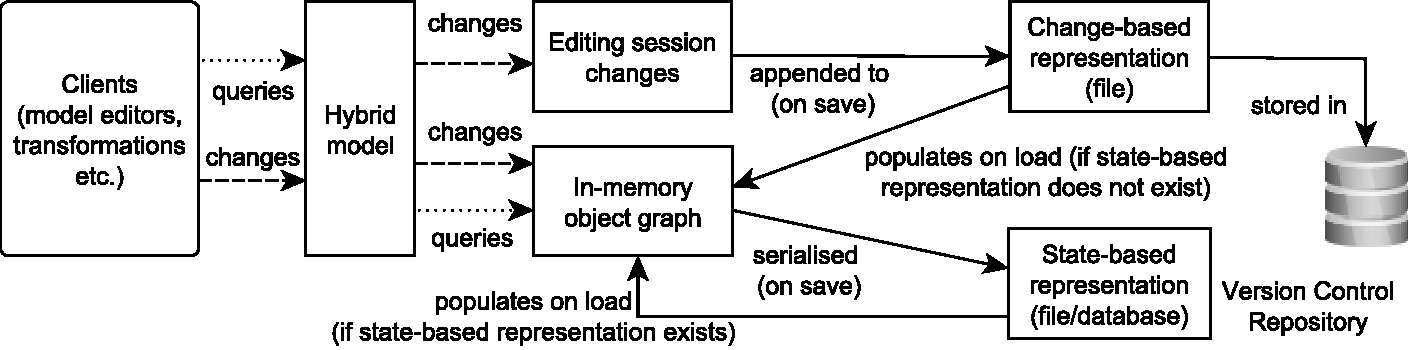
\includegraphics[width=\linewidth]{images/hybrid_persistence}
    \caption{The mechanism of hybrid model persistence.}
    \label{fig:hybrid_persistence}
\end{figure}

\textbf{Loading a hybrid model}. Models are loaded into in-memory object graphs that clients (e.g. editors, transformations) can then interact with\footnote{Depending on the state persistence mechanism, the object graph may be loaded in its entirety at startup (e.g. XMI) or loaded progressively, in a lazy manner (e.g. NeoEMF/CDO)}. In the proposed hybrid approach, if the state-based counterpart already exists, the in-memory object graph is populated from it; otherwise, it is populated by replaying the complete editing history recorded in the change-based representation.

\textbf{Changing a hybrid model}. When an element in a loaded model is created, modified or deleted, the change is applied to the in-memory object graph and is also recorded in an in-memory list of changes (\textit{Editing session changes} in Fig 2). We use the term \emph{editing session} for the period between loading a model and saving back to disk. 

\textbf{Saving a hybrid model}. The current version of the in-memory object graph is stored in the preferred state-based representation. The list of changes recorded in the current editing session (with optional processing, as described above) is appended to the change-based representation.

\textbf{Versioning a hybrid model}. Since the state-based representation is fully derived from the change-based representation, if a model needs to be versioned (e.g. in a Git repository), only the change-based representation needs to be stored. The first time it is loaded after being checked out/cloned, the state-based representation is computed and persisted locally and is used in subsequent model loading steps.

\textbf{Comparing hybrid models}. To compare two hybrid models, their change-based representations are used: this is much more efficient than state-based comparison as demonstrated in Section \ref{sec:identifying_deleted_elements}.


\subsection{Change-based Comparison}
\label{sec:change-based_comparison}

To explain our approach for change-based model comparison and merging, we present a parallel version (server version) of the change-based model in List. \ref{lst:cbpmodel} (local version). To perfoms the comparison, a client has to check whether its version is already updated up to the remote version. if it is not then the local version has to be updated first, before the local changes can be committed to the server. During the update, a model comparison is performed. Instead of only comparing the two models and present the results at the event/change level as has been done in \cite{koegel2010emfstore}, we use the information contained in the CBPs and local  SBP (since we use the hybrid approach) to reconstruct partial three structures of the models so that it can be displayed on an existing model comparison tool (e.g. EMF Compare) to help modellers identify differences visually (the three structures might not complete since limited information available).  

\begin{lstlisting}[style=eol,caption={A parallel version of the CBP in List. \ref{lst:cbpmodel}.},label=lst:cbpmodel_parallel]
session 1
create p1 type Package
set p1.name to "X" 
create c1 type Class
set c1.name to "A"
create c2 type Class
set c2.name to "B"
add c1 to p1.packagedElement 
add c2 to p1.packagedElement
session 3
set c1.name to "D"
set c2.name to "E"
create c3 type Class
set c3.name to "F"
\end{lstlisting}

Instead of loading the entire events of both change-based models, we only load both models starting from the line where they are different. They start to be different at line 10 -- $session$ $2$ (local version) and $session$ $3$ (server version). From the local model, we can identify that $c2$ has been modified -- its name has been changed to ``C'' -- and $c1$ has been removed from $p1$.$packagedElement$ and deleted. While in  the server model, we can identify $c1$ and $c2$ have been modified--both their $name$s has been changed to  ``D'' and ``E'' respectively, and also the creation of new Class $c3$. Using these information, we can determine the differences: (1) $empty$ $element$ <--> $c1$, (2) $c2$.$name$ = ``C'' <--> $c2$.$name$ = ``E'', and (3) $empty$ $element$ <--> $c3$ (left-side = local, right-side = server). The illustration can be seen in Fig. \ref{fig:comparison}.

For the right-side tree, we can determine that the right-side $c1$ and $c2$ are contained by $p1$.$packagedElement$. For $c1$, the $c1$ on the left-side are removed from the left-side $p1$. $packagedElement$ and there is no event related to $c1$ that modifies the container of $c1$ on the right-side in its session. For $c2$, its container can be determined by retrieving the information from the left-side/local SBP since we cannot find the information about its container directly from both CBPs starting from the line they are different. 

\begin{figure}
    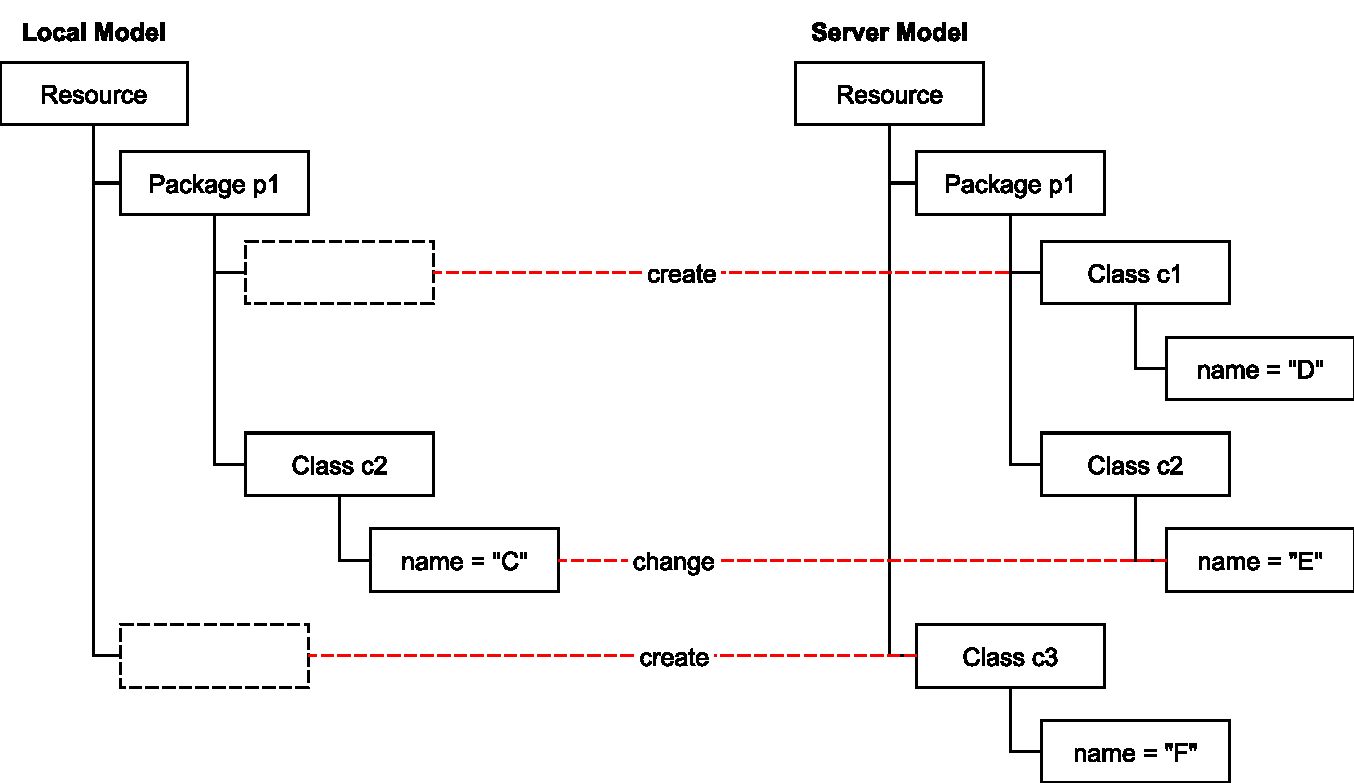
\includegraphics[width=\linewidth]{images/comparison}
    \caption{The partial comparison trees constructed from two compared change-based models.}
    \label{fig:comparison}
\end{figure}

%\subsection{Change-based Comparison}
%persist in text-based -> SVN
%Master version
%only changes are persisted into SVN
%local = change-baed vs state-based
%local-stated based are constructed using the change-based
%
%- Optimising saving and loading.
%- Hybrid model.
%- Using changes to identify differences at the structure level.


\section{Evaluation}

%\subsection{Saving Time and Memory}
%2.6 million} & \multicolumn{1}{r}{1.8 million} & \multicolumn{1}{r}{79,459
%
%between original CBP (CBP), optimised CBP (OCBP)
%
%\begin{table}[ht]
%    \footnotesize
%    \centering
%    \caption{The t-test results of saving time and memory footprint comparison after saving an event.}
%    \label{table:ttest_results_savetime}
%    \begin{tabular}
%        {| c c c | c c c c |}
%        \hline 
%        Group & Mean & SD & Comparison & t  & df & p-value \\  
%        \hline 
%        \multicolumn{7}{|c|}{Saving Time} \\
%        \hline
%        CBP & 0.00069    & 3.4e-5 & \multirow{2}{*}{CBP vs XMI} & \multirow{2}{*}{-6.01}   & \multirow{2}{*}{21.00} & \multirow{2}{*}{$<$ 0.05} \\
%        XMI & 0.40025   & 595e-5 &  &   &   &  \\ 
%        \hline
%        \multicolumn{7}{|c|}{Saving Memory Footprint} \\
%        \hline 
%        CBP & 0.0025    & 18.8e-6 &  \multirow{2}{*}{CBP vs XMI} & \multirow{2}{*}{-4.3e\texttt{+}6} & \multirow{2}{*}{21.00} & \multirow{2}{*}{$<$ 0.05} \\
%        XMI & 17.61   & 2.4e-6 &  &  &  &  \\ 
%        \hline 
%        \hline 
%    \end{tabular}
%$Mean$ = average, $SD$ = standard deviation, $t$ = t-test's $t$-$value$, $df$ = degree of freedom, $p$-$value$ = significance, $s$ = the unit is seconds
%\end{table}

\subsection{Loading Optimisation}
This section presents the evaluation results of the proposed CBP loading optimisation approach presented in Section \ref{sec:loading_and_file-size_optimisation}. We reversed the Epsilon project \cite{eclipse2017epsilon} to obtain a change-based model. The model consists of 80,000 elements and 2.6 million events which after the optimisation only 1.8 million events are effective -- other events are ignored. Using this model, we measured the performance of the optimised CBP (OCBP) on time and memory footprint of loading and saving and measured their significance using $t$-$test$. We compare the performance of OCBP against original CBP (CBP) and XMI. 

\begin{table}[ht]
    \footnotesize
    \centering
    \caption{The t-test results of loading time and memory footprint comparison after loading a model.}
    \label{table:ttest_results_loadtime}
    \begin{tabular}
        {| c c c | c c c c |}
        \hline 
        Group & Mean & SD & Comparison & t  & df & p-value \\  
         \hline 
        \multicolumn{7}{|c|}{Loading Time} \\
        \hline
        CBP & 16.60    & 0.23 &  CBP vs XMI & 324.18   &22.78 & $<$ 0.05 \\
        OCBP &  8.28  &  0.09 & CBP vs OCBP & 160.06 & 27.48 & $<$ 0.05 \\  
        XMI & 0.60   & 0.05 & OCBP vs XMI & 354.52   &42.06  & $<$ 0.05 \\ 
        \hline 
        \multicolumn{7}{|c|}{Loading Memory Footprint} \\
        \hline
        CBP &15.74    & 1.248 &  CBP vs XMI & 28.16   &  41.99 & $<$ 0.05 \\
        OCBP & 43.15   & 0.056 & CBP vs OCBP & -102.9 &21.08 & $<$ 0.05 \\  
        XMI & 5.05   & 1.271 & OCBP vs XMI & 140.49  & 21.08  & $<$ 0.05 \\ 
        \hline 
    \end{tabular}
    $Mean$ = average, $SD$ = standard deviation, $t$ = t-test's $t$-$value$, $df$ = degree of freedom, $p$-$value$ = significance, $s$ = the unit is seconds
\end{table}

The results are displayed in Table \ref{table:ttest_results_loadtime}. The table shows that OCBP outperforms original CBP on on loading time but requires more memory to perform the optimisation. However, loading the model from XMI still greatly outperforms both original and optimised CBPs. These results motivate us to perform the hybrid persistence approach.

\subsection{Hybrid Persistence}
We evaluated the performance of our hybrid persistence prototype against SBP (with NeoEMF backend) regarding time, memory footprint, storage space for loading and saving. W used the nonparametric Mann-Whitney U test with a significance level of 5\%. The model used for this evaluation was reverse-engineered from the Epsilon project. The models consist of 4.3 million change-based events and 88,020 model elements. The size of its change-based file is 406 MBs and  188 MBs for its NeoEMF backend.

As can be noticed in Table \ref{table:time_memory_footprint}, the hybrid persistence experiences a slight slowdown on loading and saving time (hybrid approach's $mean$ $>$ state-based approach's $mean$). However, the slowdown is not significant, which means that side-effect of the hybrid approach on loading and saving time is still acceptable. The hybrid approach also produces more memory footprint compared to the state-based-only approach. Nevertheless, considering the cost of main memory, this condition is acceptable in almost all real-world scenarios. The last row of the table derives an average space usage per element (for the SBP) or event (for the CBP). We can estimate the storage space usage for a hybrid persistence to be the combination of CBP and the appropriate SBP space usage.

\begin{table}[ht]
    \centering
    \begin{footnotesize}
        \caption{The comparison on time, memory footprint, and storage space for loading and saving models of the hybrid and state-based-only persistence (NeoEMF backend).}
        \label{table:time_memory_footprint}
        \begin{tabular}{ | c | c | c | c | c | c | c | c | c | }
            \hline
            \textbf{Dimension} & \multicolumn{2}{c|}{\textbf{Hybrid}} & \multicolumn{2}{c|}{\textbf{State-based}} & \multicolumn{2}{c|}{\textbf{Significance}} \\
            \hhline{~------}
            & $mean$ & $sd$ & $mean$ & $sd$ &  $W$ & $p$-$value$ \\
            \hline
            \makecell{Load Time} & 0.292 & 0.061 & 0.279 & 0.023 & 258 & \textbf{0.72}\\ 
            \hline
            \makecell{Save Time} & 0.0892 & 0.0421 & 0.0829 & 0.0494 & 216 & \textbf{0.55}\\ 
            \hline
            \makecell{Load Memory} & 38.601 & 0.878 & 10.014 & 1.088 & 0 & $<$ 0.05\\ 
            \hline
            \makecell{Save Memory} & 2.64 & 1.29 & 2.61 & 0.78 & 283 & \textbf{0.34}\\ 
            \hline
            \makecell{Storage Space} & \multicolumn{2}{c|}{\makecell{2 KBs/element\\+ 98 bytes/event}} & \multicolumn{2}{c|}{2 KBs/element} & \multicolumn{2}{c|}{---} \\ 
            \hline
        \end{tabular}
        \justify
        The time is in seconds, and the memory footprint is in MBs.
    \end{footnotesize}
\end{table}

\subsection{Identifying Deleted Elements}
\label{sec:identifying_deleted_elements}
In this section, we present the evaluation of CBP in detecting changes of models. As the scenario for the evaluation, we identify the elements in the older model that have been deleted in the newer model. We have generated a dataset of UML2 models comprises hybrid models which are reverse-engineered from the commits number 8, 44, 181, and 388 of the Epsilon project on GitHub. The description of the models can be found in Table \ref{table:version_description}.

\begin{table}[ht]
    \centering
    \caption{Description of version 8, 44, 181, and 388 of the Epsilon project's UML2 model.}
    \label{table:version_description}
    \begin{tabular}{ r r r r r}
        \hline 
        \textbf{\thead{Versions}} & \textbf{\thead{Element\\Counts}} & \textbf{\thead{Delta Elements\\(from ver. 8)}} & \textbf{\thead{Event\\Counts}} & \textbf{\thead{Delta Events\\(from ver. 8)}} \\
        \hline 
        008	& 25,993 & 0	& 90,888 & 0\\
        044	& 31,240 & 5,247	& 166,659 & 75,771\\
        181	& 34,196 & 8,203	& 250,073 & 159,185\\
        388	& 48,482 & 22,489 & 332,315 & 241,427\\
        \hline 
    \end{tabular}
\end{table}

We compare the performance between identifying the deleted elements by iterating through each events of the change-based persistence (\emph{the hybrid method}) and performing a state-based model comparison between the two compared versions using EMF Compare (\emph{the state-based method}).  As can be noticed in Fig. \ref{fig:delete_detection_epsilon_average}, identifying the deleted elements using the hybrid method is faster than the state-based method particularly when the models grows -- increase in version number, number of elements (model size), and  number of events (editing size). The change identification time of the hybrid method tends to grow linearly as the number of events increases, whereas the stated-based method tends to grow exponentially as the number of elements increases (Table \ref{table:version_description}).

\begin{figure}
    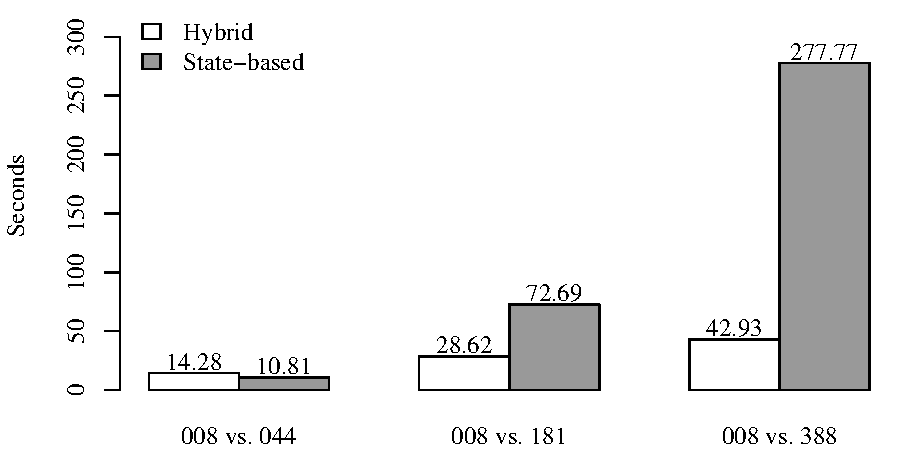
\includegraphics[width=\linewidth]{images/delete_detection_epsilon_average}
    \caption{The time required for hybrid and state-based methods on detecting deleted elements in newer versions.}
    \label{fig:delete_detection_epsilon_average}
\end{figure}

\section{Conclusions and Future Works}
In this paper, we have proposed our CBP implementation as well as our solutions to reduce its side-effects. Based on the evaluation results, the hybrid model persistence provides benefits on model loading time and change detection with an acceptable trade-off on memory footprint and storage space usage. 

Currently, we are still working on the hybrid model comparison (Section \ref{sec:hybrid_model_persistence} -- Comparing hybrid models). So far, the progress is promising. Based on our preliminary investigation, it can detect atomic changes of models faster than state-based model comparison, e.g. detecting elements that have been removed from older versions. In the future, we plan to evaluate hybrid model persistence on even larger models and perform experiments where software modellers are asked to construct change-based models. We also plan to develop a solution for the efficient merging of change-based and hybrid models. 



%% Acknowledgments
\begin{acks}                            %% acks environment is optional
This work was partly supported by through a scholarship managed by \emph{Lembaga Pengelola Dana Pendidikan Indonesia} (Indonesia Endowment Fund for Education).
\end{acks}


\bibliographystyle{ACM-Reference-Format}
\bibliography{references}

\end{document}
